% Original vector artwork for source Fig.59.1, PDF246 / printed234.
% Fermion arrows carry p1, p1-k1' (or p1-k2'), and -p2.
% Photon momentum arrows point away from the vertices.
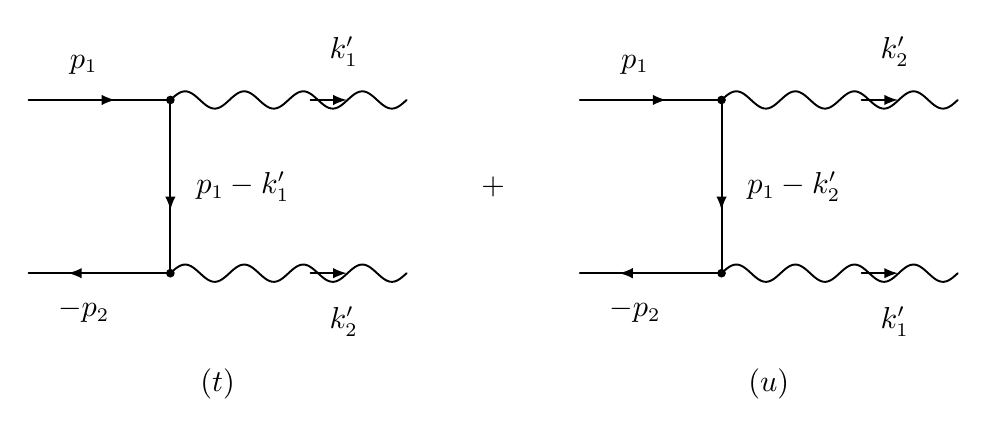
\begin{tikzpicture}[x=1mm,y=1mm,line width=.7pt,>=latex,
  line cap=round,line join=round,font=\fontsize{10.5}{12}\selectfont]
  \foreach \offset in {0,70}{
    \begin{scope}[shift={(\offset,0)}]
      \draw (0,11)--(18,11)--(18,-11)--(0,-11);
      \draw[->] (5,11)--(11,11);
      \draw[->] (18,4)--(18,-3);
      \draw[->] (11,-11)--(5,-11);
      \foreach \height in {11,-11}{
        \draw[domain=0:30,samples=101,smooth,variable=\u]
          plot ({18+\u},{\height+1.1*sin(48*\u)});
        \draw[->] (35.8,\height)--(40.4,\height);
        \fill (18,\height) circle[radius=.55mm];
      }
      \node[above] at (7,13) {$p_1$};
      \node[below] at (7,-13) {$-p_2$};
    \end{scope}
  }
  \node[right] at (20,0) {$p_1-k'_1$};
  \node[above] at (40,14) {$k'_1$};
  \node[below] at (40,-14) {$k'_2$};
  \node at (24,-25) {$(t)$};
  \node at (59,0) {$+$};
  \node[right] at (90,0) {$p_1-k'_2$};
  \node[above] at (110,14) {$k'_2$};
  \node[below] at (110,-14) {$k'_1$};
  \node at (94,-25) {$(u)$};
\end{tikzpicture}
